\documentclass[]{auvsi_doc}
\setkeys{auvsi_doc.cls}{
	AUVSITitle={Airframe Subsystem Requirements Matrix},
	AUVSILogoPath={./figs/logo.pdf}
}

\usepackage{rotating}

% include extra packages, if needed

\begin{document}

\begin{AUVSITitlePage}
\begin{artifacttable}
\entry{AF-001, 0.1, 10-23-18, Initial Draft, Tyler Critchfield \& Ryan Anderson, Derek Knowles}
\entry{AF-001, 0.2, 11-06-18, Revisions for Final Submission, Tyler Critchfield, Ryan Anderson}
% additional \entry{} commands for extra rows in the revision table, if needed
\end{artifacttable}
\end{AUVSITitlePage}

%\AUVSIFigure{figs/requirements_matrix.pdf}{0.8\textwidth}{Top-level requirements matrix for the unmanned aerial system.}{fig:reqMat}

\begin{figure}
	\centering{
		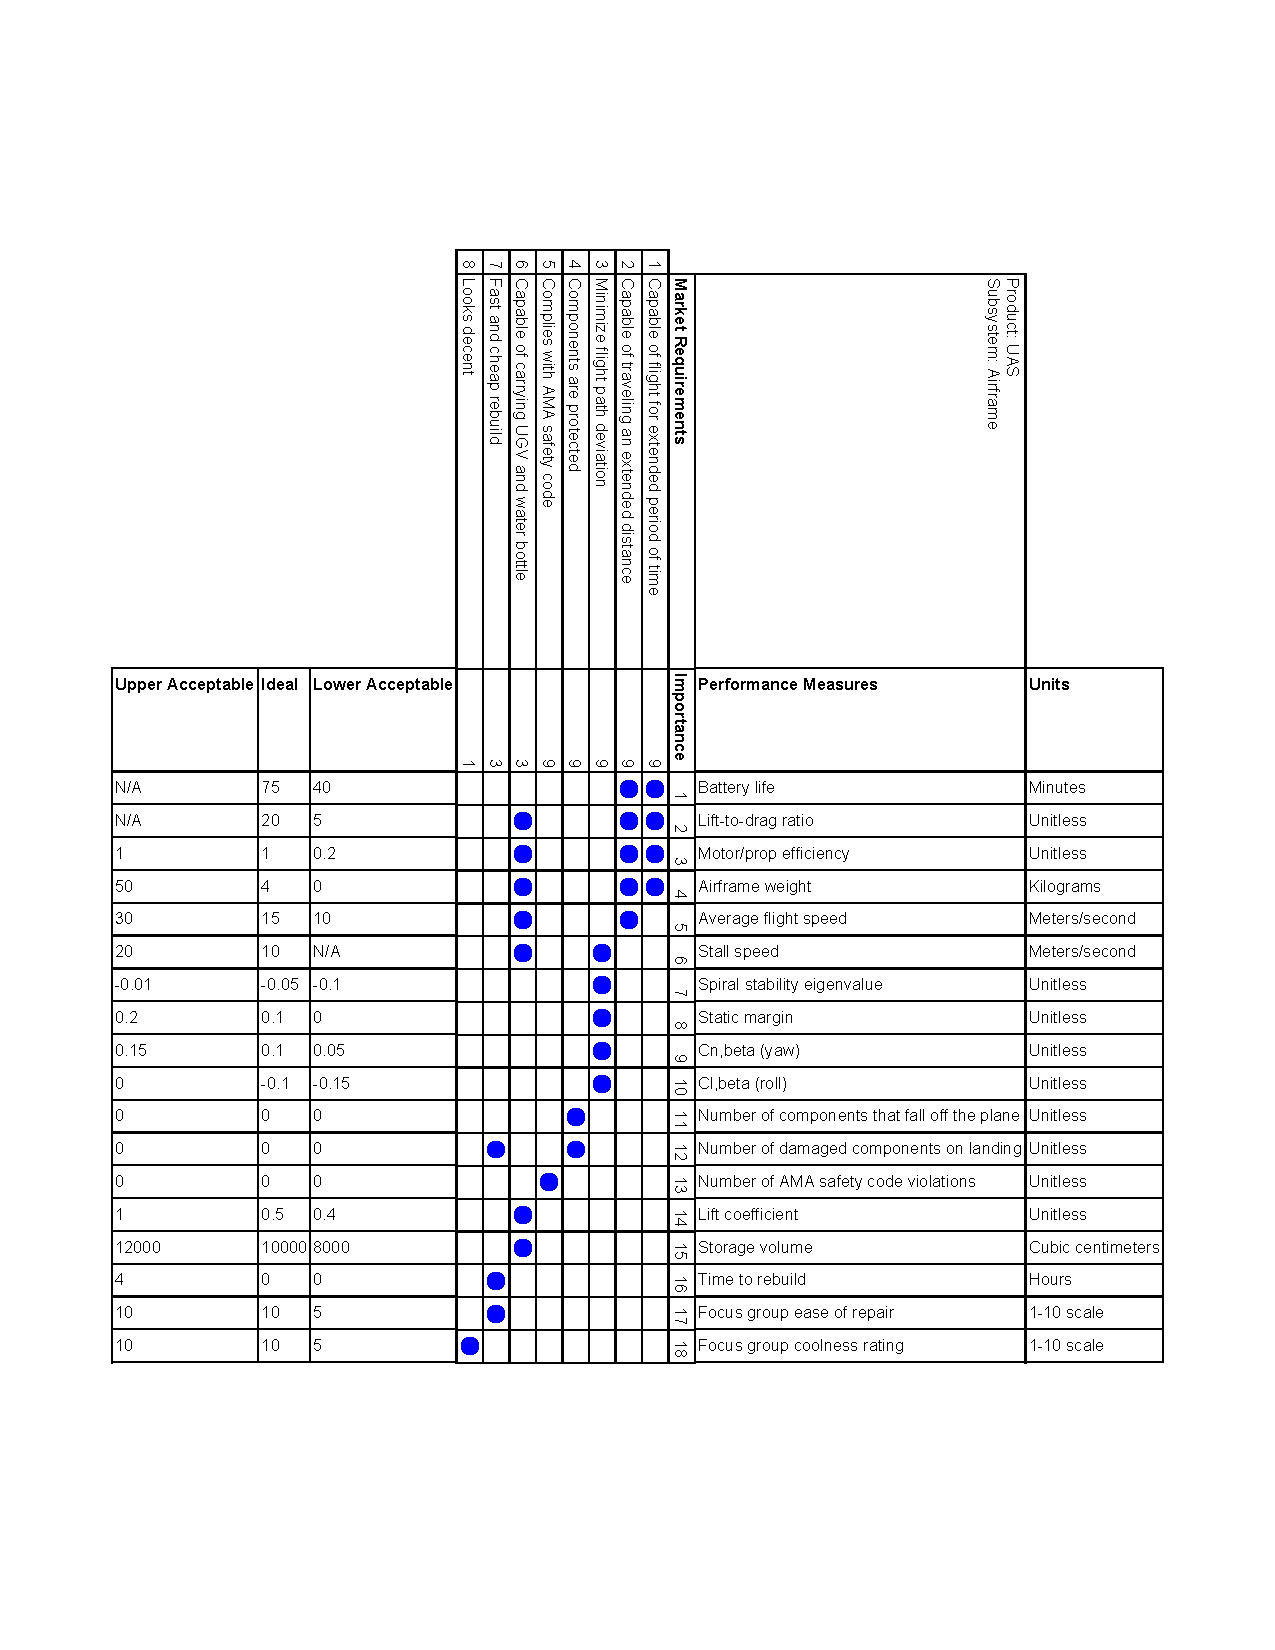
\includegraphics[width=1.3\textwidth]{figs/RequirementsMatrixAirframe.pdf}
		\captionof{figure}{Airframe subsystem requirements matrix. Note that sometimes ideal values are unrealistic; rather, they are ideal. E.g., the ideal required build time is not time at all. Realism will be incorporated into target values in a future version of the Requirements Matrix.}
		\label{fig:reqMat}}
\end{figure}

\end{document}